\subsubsection{Измерения}
8. Для начала измерены или изучены в паспорте некоторые
величны:
\begin{itemize}
    \item длина стержня -- 133 см,
    \item материал стержня -- бронза,
    \item толщина стержня -- 5.8 мм,
    \item расстояние от лазера до линейки -- 160 см,
    \item радиус диска -- 106 мм.
\end{itemize}

9. Далее измерены отклонения маятника от 0 для разных
масс (номер в первой строке -- порядковый номер измерения):
\begin{center}
\begin{tabular*}{0.75\textwidth}{@{\extracolsep{\fill}}|c|c|c|c|}
    \hline
    Вес, г & 1, мм & 2, мм & 3, мм \\
    \hline
    50 & 0 & 0 & 1\\
    \hline
    100 & 31 & 30 & 28\\
    \hline
    150 & 53 & 59 & 59\\
    \hline
    200 & 84 & 81 & 84\\
    \hline
    250 & 113 & 112 & 105\\
    \hline
    300 & 140 & 134 & 132\\
    \hline
    350 & 167 & 161 & 169\\
    \hline
    400 & 195 & 189 & 190\\
    \hline
    450 & 215 & 213 & 218\\
    \hline
    500 & 246 & 246 & 246\\
    \hline
\end{tabular*}
\end{center}

\subsubsection{Обработка}
10. Можно довльно просто посчитать угол сдвига
\begin{equation}
\varphi \approx \sin\varphi = \frac{d}{L}.
\end{equation}
Представим его в такой же таблице, что и
представлены измерения:

\begin{center}
\begin{tabular*}{0.75\textwidth}{@{\extracolsep{\fill}}|c|c|c|c|}
    \hline
    Вес, г & $\varphi$, $10^{-3}$ & $\varphi$, $10^{-3}$ & $\varphi$, $10^{-3}$ \\
    \hline
    50 & 0 & 0 & 1\\
    \hline
    100 & 19 & 19 & 18\\
    \hline
    150 & 33 & 37 & 37\\
    \hline
    200 & 52 & 51 & 52\\
    \hline
    250 & 71 & 70 & 66\\
    \hline
    300 & 88 & 84 & 82\\
    \hline
    350 & 104 & 101 & 106\\
    \hline
    400 & 122 & 118 & 119\\
    \hline
    450 & 134 & 133 & 136\\
    \hline
    500 & 154 & 154 & 154\\
    \hline
\end{tabular*}
\end{center}

10. Посчитаем момент силы $M$ для разных случаев,
пренебрегая силой трения в блоках:
\begin{equation}
    M = 2mgr,
\end{equation}
где $m$ -- масса каждого из двух грузов, $r$ -- радиус диска.

11. Построим график $m  = k\varphi$, где $k = \frac{f}{2gr}$:
\begin{figure}[H]
    \centering
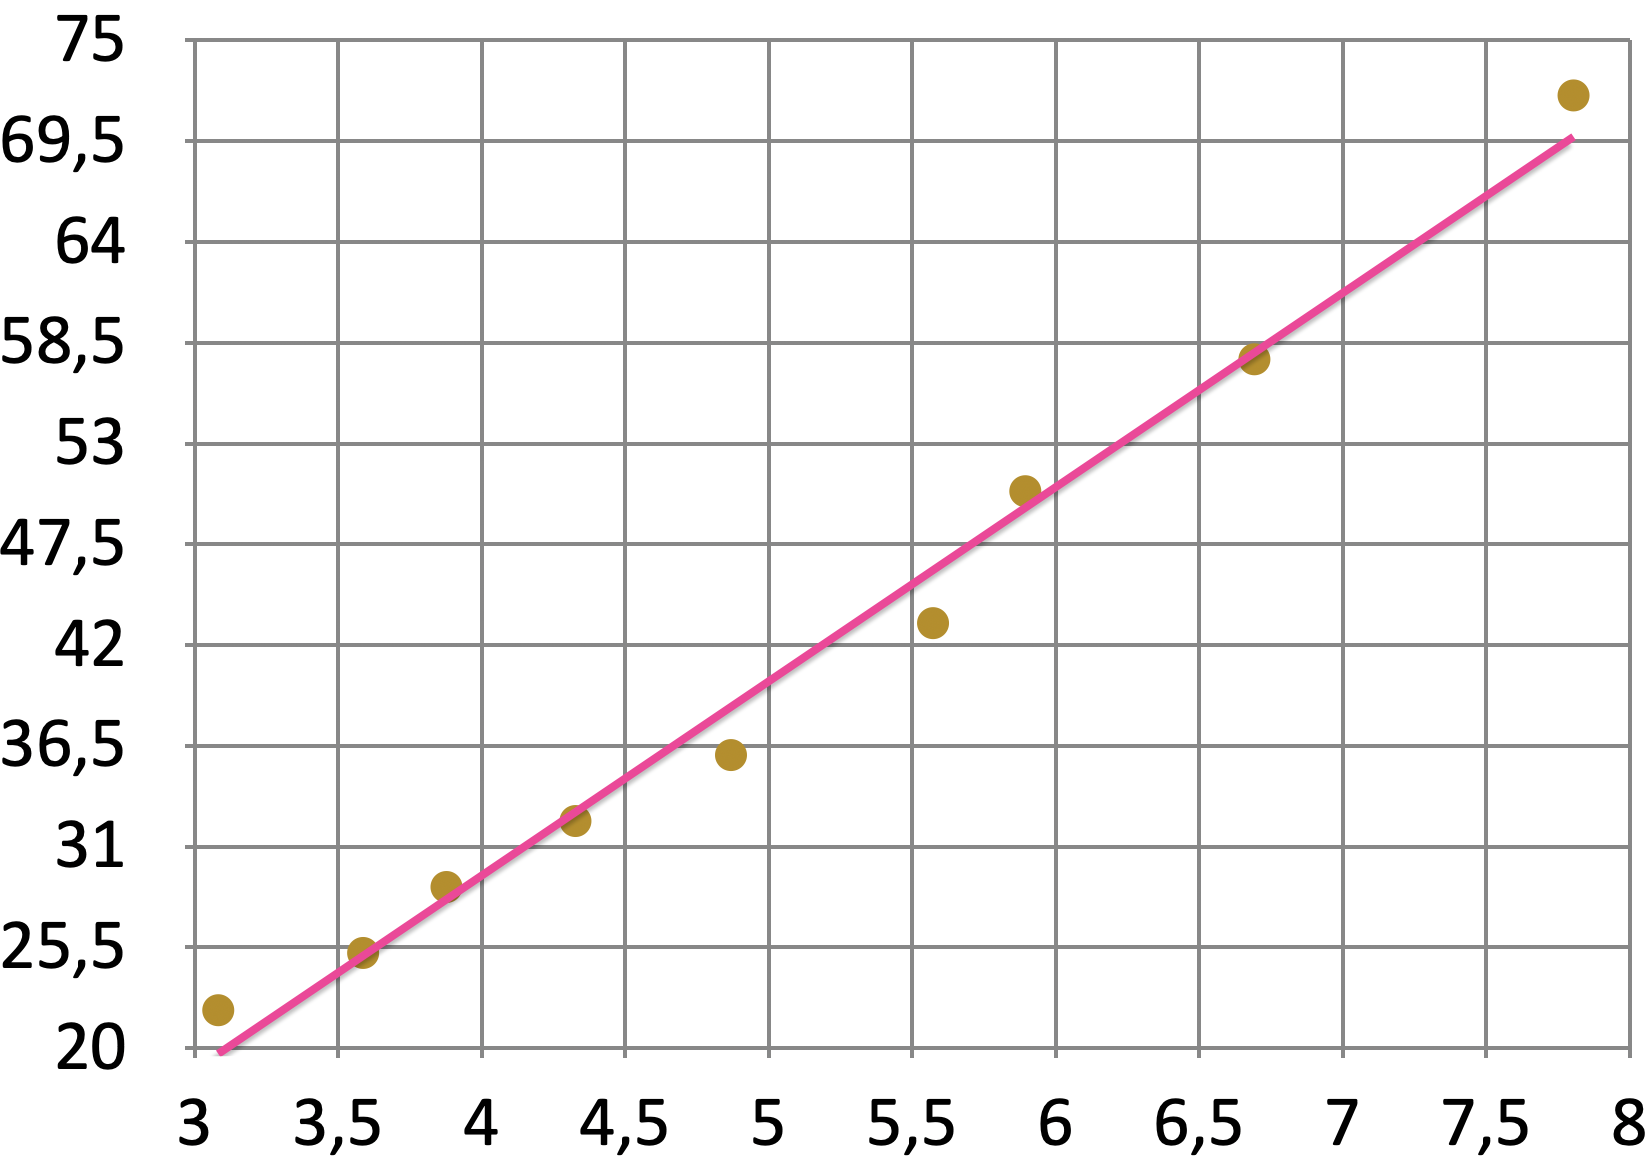
\includegraphics[width=0.75\linewidth,center]{p5.png}
    \label{fig:my_label}
\end{figure}
По графику $k = 1.86$.

12. Выразим $G$, используя форумлы (6), (15) и (16):

\[G = \frac{2lM}{\pi R^4\varphi} = \frac{4mgrl}{\pi R^4\varphi} = \frac{4grl}{\pi R^4k}.\]

Подсчет $G = 1.34 \cdot 10^{10}$ Па.
